\documentclass[10pt,aspectratio=169]{beamer}

\usetheme[progressbar=frametitle,block=fill]{metropolis}
\usepackage{appendixnumberbeamer}
\usepackage{mymacro}
%\input{Preambles/header_beamer}
%\input{Preambles/notation}


\usepackage{booktabs}
\usepackage[scale=2]{ccicons}

\usepackage{pgfplots}
\usepgfplotslibrary{dateplot}

\usepackage{amsmath}
\usepackage{amssymb}
\usepackage{amsfonts}
\usepackage{mathrsfs}
\usepackage{smartdiagram}
\usepackage{xspace}
\usepackage{fontawesome5}
\usepackage{algorithm} 
\usepackage{algpseudocode} 
\newcommand{\themename}{\textbf{\textsc{metropolis}}\xspace}

\usepackage{tikz}
\usetikzlibrary{positioning}
\usetikzlibrary{shapes,arrows}
\usetikzlibrary{decorations.pathreplacing}
\usetikzlibrary{mindmap,trees,backgrounds}
\tikzset{%
  block/.style    = {draw, thick, rectangle, minimum height = 1em,
    minimum width = 3em },
  sum/.style      = {draw, circle, node distance = 1cm}, % Adder
  input/.style    = {coordinate}, % Input
  output/.style   = {coordinate}, % Output
     invisible/.style={opacity=0},
    visible on/.style={alt={#1{}{invisible}}},
    alt/.code args={<#1>#2#3}{%
      \alt<#1>{\pgfkeysalso{#2}}{\pgfkeysalso{#3}} % \pgfkeysalso doesn't change the path
    }
  
}  


%\date{}

\titlegraphic{\hfill\includegraphics[height=1cm]{electoral_politics/gphb/EU_hz_280.png}}
\usepackage{textpos}


\setbeamertemplate{itemize item}{\color{UniGold}$\bullet$}
%\setbeamertemplate{frame footer}{Ortiz \& Sant'Anna}
\addtobeamertemplate{frametitle}{}{%
\begin{textblock*}{10mm}(.88\textwidth,-.8cm)
\includegraphics[height=0.55cm]{electoral_politics/gphb/EU_hz_rev.png}
\end{textblock*}}

\setsansfont{Noto Sans}
\setmonofont{Noto Sans Mono}

%\logo{\includegraphics[height=1cm]{}}

\definecolor{UniBlue}{RGB}{0,36,125}
\definecolor{UniGold}{RGB}{137,118,75}
\definecolor{UniGold2}{RGB}{230,176,18}
\definecolor{UniGray}{RGB}{201,201,196}
\definecolor{UniGray2}{RGB}{148,148,143}
\definecolor{UniBlue2}{RGB}{0,48,130}
\definecolor{Uniwhite2}{RGB}{255,255,255}
\definecolor{shaders}{HTML}{d7d3d3}
\definecolor{emoryblue}{RGB}{1, 33, 105}
\definecolor{emoryyellow}{RGB}{242, 169, 0}
\definecolor{emorygold}{RGB}{181, 133, 0}
\definecolor{emorymgold}{RGB}{132, 117, 78}
\definecolor{emorylblue}{RGB}{0, 125, 186}
\definecolor{emorymblue}{RGB}{0, 51, 160}

\definecolor{sBl0}{HTML}{004757}
\definecolor{sBl1}{HTML}{ffaa00}
\definecolor{sBl2}{HTML}{ff8100}
\definecolor{sBl3}{HTML}{4c9141}
\definecolor{sBl4}{HTML}{ff5100}
\definecolor{sBl5}{HTML}{0055ff}

\definecolor{arr1}{HTML}{2000ff}
\definecolor{arr2}{HTML}{ff0043}


\setbeamercolor{progress bar}{fg=UniGold }
\setbeamercolor{alerted text}{fg=emorygold}

\setbeamercolor{title separator}{fg=UniGold }
\setbeamercolor{progress bar in head/foot}{ fg=UniGold}
\setbeamercolor{progress bar in section page}{ fg=UniBlue }
%\setbeamercolor{title}{fg=UniBlue}
\setbeamercolor{frametitle}{bg=UniBlue2}
\setbeamercolor{structure}{fg=UniBlue2}
\setbeamercolor{titlelike}{fg=UniBlue}

%\setbeamercolor{block title alerted}{fg=Uniwhite2,bg=UniGray2}
%\setbeamercolor{block body alerted}{bg=UniGray,fg=UniBlue2}
%\setbeamercolor{block body default}{bg=UniGray}

\setbeamercolor{progress bar}{fg=emoryblue,bg=emoryyellow }
\setbeamercolor{title separator}{fg=emoryblue, bg=emoryblue}
% ------------------------------------------------------------------------------
% Blocks
% ------------------------------------------------------------------------------
\setbeamercolor{block body alerted}{bg=alerted text.fg!10}
\setbeamercolor{block title alerted}{bg=alerted text.fg!20}

%\setbeamercolor{block body}{bg=structure!10}
%\setbeamercolor{block title}{bg=structure!20}
%\setbeamercolor{block body example}{bg=green!10}
%\setbeamercolor{block title example}{bg=green!20}

\setbeamercolor{block body}{bg=emoryyellow!3!white, fg = black}
\setbeamercolor{block title}{bg=emorygold, fg = white}
\setbeamercolor{block body example}{bg=emoryyellow!3!white, fg = blac}
\setbeamercolor{block title example}{bg=emorygold, fg = white}

\setbeamertemplate{blocks}[rounded][shadow]
%\setbeamercolor{block body alerted}{bg=UniGray,fg=UniBlue}
\setbeamertemplate{itemize item}{\color{emoryyellow} \footnotesize{$\blacksquare$}}
\setbeamertemplate{itemize subitem}{\color{emoryyellow}\scriptsize{$\blacktriangleright$}}
%\setbeameroption{show notes on second screen=right}

\newcommand\YUGE{\fontsize{48}{60}\selectfont}

\begin{document}

\title{%
\textcolor{emoryblue}{\textbf{%
\resizebox{0.95\linewidth}{!}{The Moral Revolution Will Not Be Televised, It Will Be Livestreamed:}%
\\
Censorship and Narrative Control in Mexico}}}
\author[Joaquín Barrutia Álvarez]{\vspace{-.1cm} 
\begin{columns}
    \column{\linewidth}
    \centering
   \textcolor{emorygold}{\textbf{Joaquín Barrutia Álvarez}}  %\linebreak  \medskip Emory University
\end{columns}
\vspace{1cm}
}

\titlegraphic { 
\begin{tikzpicture}[overlay,remember picture]
\node[xshift=0cm, yshift=-.6cm] at (current page.center){
    \includegraphics[width=3cm]{electoral_politics/gphb/EU_hz_280.png}
};
\end{tikzpicture}
}
\date{\vspace{1.5cm} 
\centering
\textcolor{emorygold}{\textbf{\today}} \linebreak
}
\vspace{2cm}


\maketitle


%--------------------------------------------------------------------------------------------------------
% START WRITING YOUR PRESENTATION
%--------------------------------------------------------------------------------------------------------
\begin{frame}{Why Governments Hold Interactions with Media?}
\begin{itemize}
  \setlength\itemsep{1em}

    \item Globally, governments increasingly trying to speak \alert{directly} to audiences and to \alert{manage press access} through controlled formats (press pools, livestreams, social media).

  \item Following his 2018 victory, President L\'opez Obrador (AMLO) created a direct-to-public communication channel: the \textbf{\textit{Mañanera}}.

  \item The \textit{Mañanera} is a daily agenda-setting press conference where access to the microphone depends heavily on \textbf{visibility and physical proximity} (front rows).

  \item Initially, a ``first-come, first-served'' rule generated \textbf{adverse selection of questioners}: front-row access became concentrated among aligned outlets, limiting critical questioning and undermining perceived credibility.

  \item In April 2022, the administration introduced a \alert{daily seat lottery} for the first three rows to broaden access and restore engagement.
\end{itemize}
\end{frame}

\begin{frame}
    \begin{figure}
        \centering
        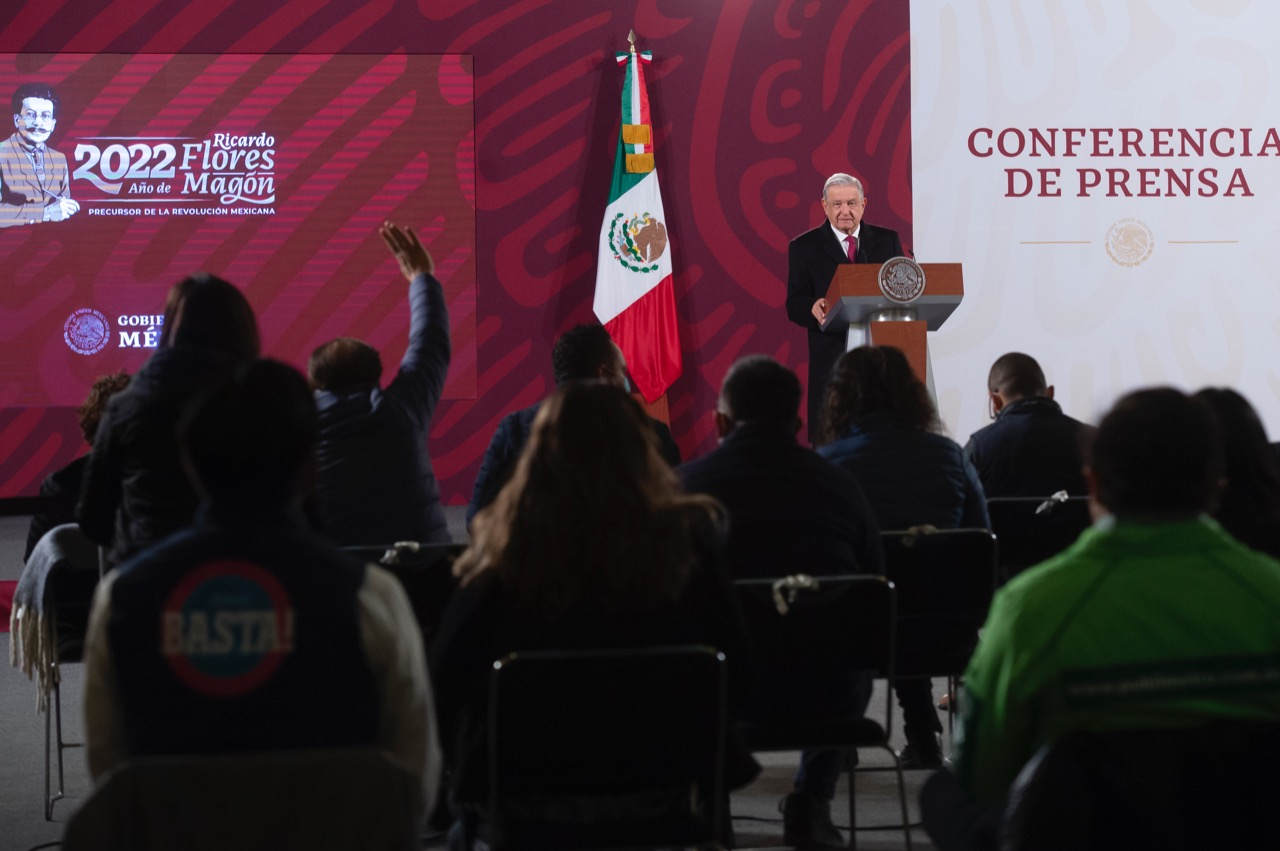
\includegraphics[width=.8\textwidth]{figures/descriptive_stats/mañanera_ex.jpeg}
        \vspace{-0.2cm}
        \caption{\scriptsize Example of a Mañanera}
    \end{figure}
\end{frame}

\begin{frame}
    \begin{figure}
        \centering
        \includegraphics[width=1\textwidth]{figures/descriptive_stats/engagement_three_panels_side_by_side_k7.png}
        \vspace{-0.2cm}
        \caption{\scriptsize The engagement dip that preceded randomized seating.}
    \end{figure}
\end{frame}

\begin{frame}{Research Questions}
\begin{itemize}\setlength\itemsep{0.95em}

\item \textbf{RQ1 (Credibility via dissent):}\\
\textit{Does committing to some dissent make government communication more credible to viewers?}
\begin{itemize}\setlength\itemsep{0.25em}
  \item \textbf{Hypothesis:} A mechanism that forces occasional critical questions---rather than a fully scripted show---\alert{raises audience engagement} by making the information environment more believable.
\end{itemize}

\pause
\vspace{0.5cm}

\item \textbf{RQ2 (Discipline via advertising):}\\
\textit{Once government allows dissent, does it use public resources to steer how much criticism those outlets supply?}
\begin{itemize}\setlength\itemsep{0.25em}
  \item \textbf{Hypothesis:} When randomly selected outlets ask more critical questions, they \alert{subsequently receive less government advertising}, consistent with a discipline rule that fine-tunes the equilibrium level of dissent.
\end{itemize}

\end{itemize}
\end{frame}



\begin{frame}{Preview: How I answer these questions}
\hypertarget{preview}{}

\textbf{Theory (Mechanism: credibility vs.\ discipline):}\\
When viewers are skeptical, a fully scripted conference is discounted as propaganda. 
A random seat lottery commits the government to occasionally letting dissent on air (boosting credibility), 
while state advertising then adjusts the incentives of those randomly selected outlets, fine-tuning the equilibrium level of dissent.
\hfill\hyperlink{appmodel}{\beamerbutton{Simple model}}
\end{frame}

\begin{frame}{Preview: How I answer these questions}
\centering
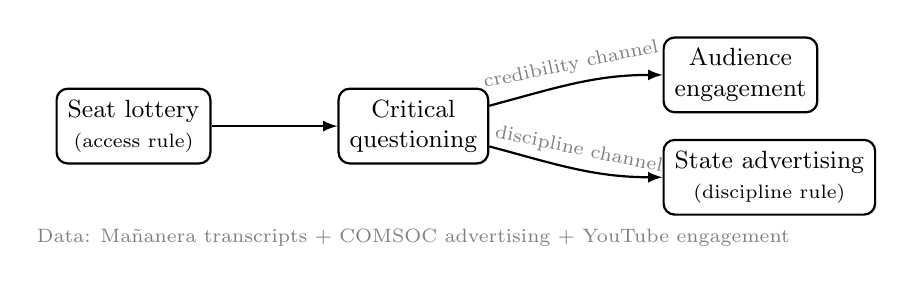
\begin{tikzpicture}[
  node distance=1.6cm,
  baseline,
  every node/.style={font=\small},
  box/.style={draw, rounded corners, thick, inner sep=4pt, align=center},
  >=latex
]
\node[box] (seat) {Seat lottery\\\scriptsize (access rule)};
\node[box, right=of seat] (q) {Critical\\questioning};
\node[box, right=2.2cm of q, yshift=0.65cm] (ads) {Audience\\engagement};
\node[box, right=2.2cm of q, yshift=-0.65cm] (eng) {State advertising\\\scriptsize (discipline rule)};

\draw[->, thick] (seat) -- (q);

\draw[->, thick]
  (q) to[out=15,in=180]
  node[midway, above, sloped, font=\scriptsize, text=gray]{credibility channel}
  (ads);

\draw[->, thick]
  (q) to[out=-15,in=180]
  node[midway, above, sloped, font=\scriptsize, text=gray]{discipline channel}
  (eng);

\node[below=0.7cm of q, font=\scriptsize, text=gray]
{Data: Ma\~nanera transcripts + COMSOC advertising + YouTube engagement};
\end{tikzpicture}

\vspace{0.5cm}

These IV estimates are not separate from the model. They pin down the key structural primitives of the persuasion mechanism: Government marginal benefit for engagement (through interaction metrics), and the marginal cost of on-air dissent (through future advertising allocations).

\end{frame}



\begin{frame}{Roadmap}
I will try to convince you of a few things: 
\begin{enumerate}\setlength\itemsep{0.7em}
  \item  Why the information environment matters for accountability, and why governments have strong incentives to shape media coverage and public narratives.
  \pause
  \item Why Mexico is a particularly relevant setting to study these questions, especially given the historical role of state advertising and the rise of the \textit{Mañanera}.
  \pause
    \item Why the seat lottery can plausibly help me answer my RQs.
\end{enumerate}
\end{frame}



%--------------------------------------------------------------------------------------------------------
% NEW SLIDE 1: THEORETICAL MOTIVATION
%--------------------------------------------------------------------------------------------------------

\section{Why this is important?}

% --- First slide in section: Why this is important? ----------------------------

\begin{frame}{Why the Information Environment Matters}
\begin{itemize}
    \setlength\itemsep{0.65em}

    \item \textbf{Media increases accountability}
    by lowering information frictions, media reporting helps voters \alert{detect} misbehavior and \alert{sanction} incumbents {\footnotesize\color{gray}\citep{Audits-Ferraz-QJE}}.

\item \textbf{Governments spend substantial resources on narrative control} {\footnotesize\color{gray}\citep{ArgCorr-DiTella-AEJAE, MediaCaptures-Zeidl-Econometrica, CensorshipChina-King-Science}}.

    \begin{itemize}
        \item Incumbents understand that
    political survival is linked to what information becomes \alert{salient} and how it is interpreted {\footnotesize\color{gray}\citep{Autocracy-Guriev-JPE}}.
    \item However, persuasion works when \alert{audiences
trust} the information environment {\footnotesize\color{gray}\citep{MediaBias-Gentzkow-JPE}}.
    \end{itemize}
    

    \item \textbf{In autocracies, the playbook is familiar:} \alert{censorship} + \alert{coercion}.
    \begin{itemize}
        \item \textit{Censorship:} China’s online censorship on collective action {\footnotesize\color{gray}\citep{CensorshipCollective-King-APSR}}.
        \item \textit{Coercion:} the murder of Jamal Khashoggi in a Saudi consulate.
    \end{itemize}
\end{itemize}
\end{frame}

\begin{frame}
\frametitle{Censorship in democracies}

\begin{itemize}
 \item \textbf{What about in democracies?}
    Direct repression is costly and often constrained, but government still has techniques to silence critics {\footnotesize\color{gray}\citep{Censor-Pratt-AER}}.
    \vspace{0.2cm}
\item Which instruments are used?

\begin{enumerate}
    \item \textbf{Bribery:} Montesinos in Peru {\footnotesize\color{gray}\citep{Peru-Macmillan-JEP}}.
    \item \textbf{De-legitimization:} South Korea \textit{giraegi} and Trump in US {\footnotesize\color{gray}\citep{KoreaJour-Shin-Journalism, PressCriticism-Carlson-Journalism}}.
    \item \textbf{Restriction of source access:} Kisha clubs in Japan {\footnotesize\color{gray}\citep{Kisha-Freedom}}.
    \item \textbf{Public resource allocation:} Argentina and Hungary governments use \alert{advertising} to \alert{reward} supportive outlets and \alert{discipline} critics {\footnotesize\color{gray}\citep{ArgCorr-DiTella-AEJAE, MediaCaptures-Zeidl-Econometrica}}.
\end{enumerate}

\vspace{0.2cm}
\item \textbf{How effective are they?}
\begin{itemize}
  \item \alert{Not Clear!} We rarely observe clean exogenous variation in exposure to dissent and government responses, causal identification is rare for most of these.
\end{itemize}
\end{itemize}
\end{frame}

\begin{frame}{What this paper adds}
\begin{itemize}\setlength\itemsep{0.85em}

  \item \textbf{Main contribution:}
  I show AMLO effectively implements a \alert{simple persuasion mechanism}:
  a \textbf{seat lottery} that commits to letting some dissent onto the air, combined with \textbf{state advertising}
  that disciplines how much dissent randomly selected outlets are willing to supply.
  This jointly shapes the information structure faced by citizens
  {\footnotesize\color{gray}\citep{MediaBias-Gentzkow-JPE}}.

\end{itemize}
\end{frame}

\begin{frame}{What this paper adds (Cont.)}
\begin{itemize}\setlength\itemsep{0.85em}

\item \textbf{Why the literature gets stuck:}
  \begin{itemize}\setlength\itemsep{0.25em}
    \item \textbf{Dissent is usually endogenous:} aligned outlets self-select into access and favorable treatment
    {\footnotesize\color{gray}\citep{ArgCorr-DiTella-AEJAE}}.
    \item \textbf{Credible commitment is hard to observe:} we rarely see reforms that plausibly change
    \textit{who can speak} and \textit{how they are rewarded} in a way that can be brought to the data.
    \item \textbf{Credibility is hard to measure:} we rarely observe clean proxies for audience attention in government messaging
    {\footnotesize\color{gray}\citep{PersuasionEmpirical-Dellavigna-AR}}.
  \end{itemize}
  
  \item \textbf{What my setting lets me do:}
  A daily seat lottery provides quasi-random variation in \alert{access to the mic},
  and rich administrative data let me trace its consequences. I estimate the causal effect of \textbf{critical questioning} on:
  \begin{itemize}\setlength\itemsep{0.25em}
    \item \textbf{audience engagement} (credibility channel, via YouTube metrics), and
    \item \textbf{state advertising} (discipline channel, via COMSOC contracts).
  \end{itemize}
\end{itemize}




\end{frame}


\section{Why Mexico?}

\begin{frame}{Mexican Context: Public Money \& Access as Control}

\begin{itemize}
    \setlength\itemsep{0.55em}

    \item \textbf{Mexico is a natural setting to study democratic censorship:}
    official advertising has long been used to \alert{reward} friendly coverage and \alert{discipline} critics.

\end{itemize}

\vspace{0.2cm}
\begin{quote}
\centering
``Pay for them to beat up on me? Gentlemen, I think not!''

\hfill --- \tiny{President L\'opez Portillo (1982), announcing the withdrawal of advertising from independent media \citep{PrensaVendida-Rod}.}
\end{quote}

\begin{itemize}
    \setlength\itemsep{0.55em}

    \item \textbf{This playbook persisted into modern electoral politics:}
\end{itemize}

\vspace{0.2cm}
\begin{quote}
\centering
``With its enormous advertising budget, Mexican government controls the media.''

\hfill --- \tiny{\citep{Times}.}
\end{quote}

\begin{itemize}
    \setlength\itemsep{0.55em}

    \item \textbf{AMLO reshaped the information environment}
    by sharply cutting official advertising and simultaneously creating the \alert{ma\~nanera}.
\end{itemize}

\end{frame}

\begin{frame}
    \begin{figure}
        \centering
        
\includegraphics[width=.6\textwidth]{figures/descriptive_stats/ppto_article19.pdf}
        \vspace{-0.2cm}
        \caption{\scriptsize Official advertising spending. Source: COMSOC.}
    \end{figure}
\end{frame}

\section{Empirics: Data and Design}

\begin{frame}{Data: what I observe on each conference day}
\begin{itemize}
  \setlength\itemsep{0.75em}

  \item I observe (i) who attends and where they sit\footnote{\scriptsize Seat-location data are pending resolution with the government.}, (ii) who asks questions, and (iii) the transcript content of those questions.


  \item I connect my two research questions to two observable outcomes:
\begin{itemize}
\setlength\itemsep{0.45em}
  \item \textbf{Engagement (conference level):}
  For each \textit{mañanera}, I collect \alert{YouTube video-level metrics} from
  (i) official government channel that livestreamed the conference and
  (ii) media outlets that simultaneously restream it.
  
  \item \textbf{Discipline (outlet-time level):}
  I use COMSOC’s administrative records on official advertising.
  These data report government ad purchases and the recipient outlet, with monetary amounts and time identifiers.
\end{itemize}

\end{itemize}
\end{frame}

\begin{frame}{How the Seat Lottery Works}
\begin{itemize}
  \setlength\itemsep{0.8em}

  \item After April 2022, access to the \alert{first three rows} started depending on \alert{daily lottery} among accredited attendees.

  \item The lottery is \alert{stratified by media type}: seats are drawn separately within categories (e.g., print, TV, radio, digital), and then assigned to the front rows.

  \item Rotation rule: outlets that asked a question the day before are excluded from the lottery.

  \item My identifying claim is simple: \alert{within day $\times$ media type $\times$ not-asked-yesterday}, who lands in the first rows is as-good-as random.
\end{itemize}
\end{frame}

\begin{frame}{Relevance: lottery shifts who gets the mic and what gets aired}
\small
\begin{itemize}\setlength\itemsep{0.65em}

  \item \textbf{Seat location predicts voice.}
  In a hand-coded sample of 10 randomly selected conferences, the distribution of questions by row is:
  \[
  \text{Row 1: }71\% \quad\text{Row 2: }20\% \quad\text{Row 3: }4.5\% \quad\text{Other: }4.5\%.
  \]

  \item \textbf{Implication: it shifts the on-air ``question market.''}
  If being in the first rows is the main bottleneck, randomizing those seats should:
  \begin{itemize}\setlength\itemsep{0.35em}
    \item \alert{deconcentrate} question access (fewer outlets monopolizing the mic), and
    \item increase the probability that \alert{more critical outlets} are the ones whose questions become salient on air.
  \end{itemize}

  \item \textbf{What this buys me empirically:}
  lottery-induced variation in \emph{who} gets front-row visibility generates quasi-random variation in \emph{who} gets to ask, hence in \emph{critical content} reaching viewers.

\end{itemize}
\end{frame}

\begin{frame}
  \centering
  
\includegraphics[width=\linewidth]{figures/descriptive_stats/outlet_density2.pdf}

  \vspace{0.4em}
  \scriptsize
  \begin{tabular}{l}
  \end{tabular}

\vspace{0.35em}
\centering
\scriptsize
% If the table is too large, keep it as a separate slide. If it fits, include it here:
% \vspace{0.2em}
% \input{tables/top10_outlets_before_after.tex}
\end{frame}




\begin{frame}

\begin{table}[!htpb]
    \centering
    \scriptsize
    \caption{Top 10 Outlets that Asked the Most Questions}
    \label{tab:outlets}
    \begin{tabular}{cccc}
\hline \\
Outlet (Before) & Questions (Before) & Outlet (After) & Questions (After) \\
\hline\\
Grupo Healy & 72 &  Grupo Healy & 32 \\
 A Tiempo TV  & 42 &  La Crónica & 31 \\
 Tabasco Hoy & 40 & Frontera & 30 \\
 Campeche Hoy & 39 &  Contralínea & 29 \\
 Quintana Roo Hoy\footnote{\tiny Widely considered 'southern friendly outlets' of the government (\href{https://animalpolitico.com/verificacion-de-hechos/te-explico/amlo-medios-promesas-publicidad-oficial}{Animal Político})} & 37 &  SDP Noticias & 28 \\
Frontera & 35 &  Proceso\footnote{\tiny AMLO of Proceso: '\textit{Conservative journalism, serving corrupt minorities, either directly or indirectly, consciously or unconsciously.}'}  & 28 \\
 diario Basta\footnote{\tiny Diario Basta CEO: 'Thanks to my friend and fellow countryman, President López Obrador, for his support throughout his administration to @diariobasta and @grupocanton. Love is repaid with love.'} & 33 &  Canal 11 & 25 \\
 La Crónica & 32 &  El Financiero\footnote{\tiny AMLO to a Financiero journalist: '\textit{I don't want to get involved in that. Why should I give a story to your newspaper if you're against us?}'} & 22 \\
 Contralínea & 29 &  Noticiero en Redes. & 18 \\
 Imagen del Golfo  & 28 &  Tabasco Hoy & 16 \\
\hline
\end{tabular}
\end{table}
\end{frame}


{\setbeamercolor{palette primary}{fg=gray, bg=white}
\begin{frame}[standout]

Thanks!\\

\small  \faIcon{envelope} joaquin.barrutia.alvarez@emory.edu \\
\small \faIcon{link} https://quinoba.github.io/ \\
\end{frame}
}

\begin{frame}[allowframebreaks]
    \printbibliography
\end{frame}


%--------------------------------------------------------------------------------------------------------
% APPENDIX: THEORETICAL MODEL
%--------------------------------------------------------------------------------------------------------
\appendix

\section*{Appendix}

\begin{frame}{Appendix: A Simple Bayesian Persuasion Model}
\hypertarget{appmodel}{}
\label{appmodel}

\textbf{Setup: The Government (Sender) and the Public (Receiver)}

\begin{itemize}
    \setlength\itemsep{0.8em}
    \item \textbf{State of the World:} $\theta \in \{G, B\}$ (Good, Bad).
    \item \textbf{Prior Belief:} $q = \Pr(\theta = G)$.
    \item \textbf{Public's Action:} $a \in \{0, 1\}$ (Disengage, Support).
    \begin{itemize}
        \item The public supports ($a=1$) iff belief $\Pr(G \mid m) \ge \tau$ (credibility threshold).
    \end{itemize}
    \item \textbf{Assumption (Skepticism):} $q < \tau$. 
    \begin{itemize}
        \item \footnotesize{The government starts with a credibility deficit. Without new information, the public disengages.}
    \end{itemize}
    \item \textbf{Signal (The Broadcast):} $m \in \{S, O\}$.
    \begin{itemize}
        \item $S$: \textbf{Scripted} (Only favorable questions).
        \item $O$: \textbf{Open} (Critical dissent is visible).
    \end{itemize}
\end{itemize}

\end{frame}

\begin{frame}{Why Total Censorship Fails}

Suppose the government chooses \textbf{Total Control}: always produce a Scripted broadcast ($S$), regardless of the state.

\vspace{0.3cm}

\begin{itemize}
    \item \textbf{Information Structure:}
    \[ \Pr(S \mid G) = 1, \quad \Pr(S \mid B) = 1 \]
    
    \item \textbf{Public's Inference (Bayes' Rule):}
    Since the message is uninformative, the posterior equals the prior:
    \[ \Pr(G \mid S) = q \]
    
    \item \textbf{Outcome:}
    Since $q < \tau$ (Skepticism), the public chooses $a=0$ (Disengage).
    
    \item \textbf{Result:} 
    \alert{Total censorship yields zero political support.} The broadcast is discounted as "pure propaganda."
\end{itemize}

\end{frame}

\begin{frame}{The Optimal Solution: Interior Dissent}

The government maximizes the probability of Support ($a=1$) by choosing a signal structure $\beta = \Pr(S \mid B)$ (how often to hide the Bad state).

\vspace{0.2cm}

\textbf{Optimal Strategy:}
\begin{enumerate}
    \item Always show Scripted if things are Good: $\Pr(S \mid G) = 1$.
    \item Choose $\beta < 1$ such that the "Scripted" signal is \textit{just credible enough}:
    \[ \Pr(G \mid S) = \frac{q \cdot 1}{q \cdot 1 + (1-q) \cdot \beta} = \tau \]
\end{enumerate}

\vspace{0.2cm}
\textbf{The Interior Solution:}
\[ \beta^* = \frac{q}{1-q} \frac{1-\tau}{\tau} < 1 \]

\vspace{0.2cm}
 To maximize support, the government \textbf{must allow some dissent} ($\Pr(O \mid B) > 0$). The optimal level of censorship is interior, not absolute.


\centering
\hyperlink{preview}{\beamerbutton{Back to Main Presentation}}

\end{frame}

\end{document}